\documentclass[10pt]{book}

% --- KDP 6x9 MIT Bleed: Seite = 6.125" x 9.25" ---
\usepackage[
paperwidth=6.125in,
paperheight=9.25in,
margin=0in
]{geometry}

% --- Pakete ---
\usepackage[pages=all]{background}
\usepackage{graphicx}
\usepackage{tikz}
\usetikzlibrary{calc}
\usepackage{xcolor}
\usepackage{anyfontsize}
\usepackage[protrusion=true,expansion=true]{microtype}

\pagestyle{empty}
\setlength{\parindent}{0pt}

% --- Farben ---
\definecolor{coveraccent}{HTML}{00B7C2} % Akzentfarbe
\definecolor{covertext}{HTML}{E6E6E6}   % heller Fließtext

% --- Hintergrundbild ---
% Ideal: 300 dpi bei 6.125"x9.25" ca. 1838 x 2775 px
% Datei muss im gleichen Ordner liegen wie diese .tex-Datei.
\backgroundsetup{
	scale=1,
	angle=0,
	opacity=1,
	contents={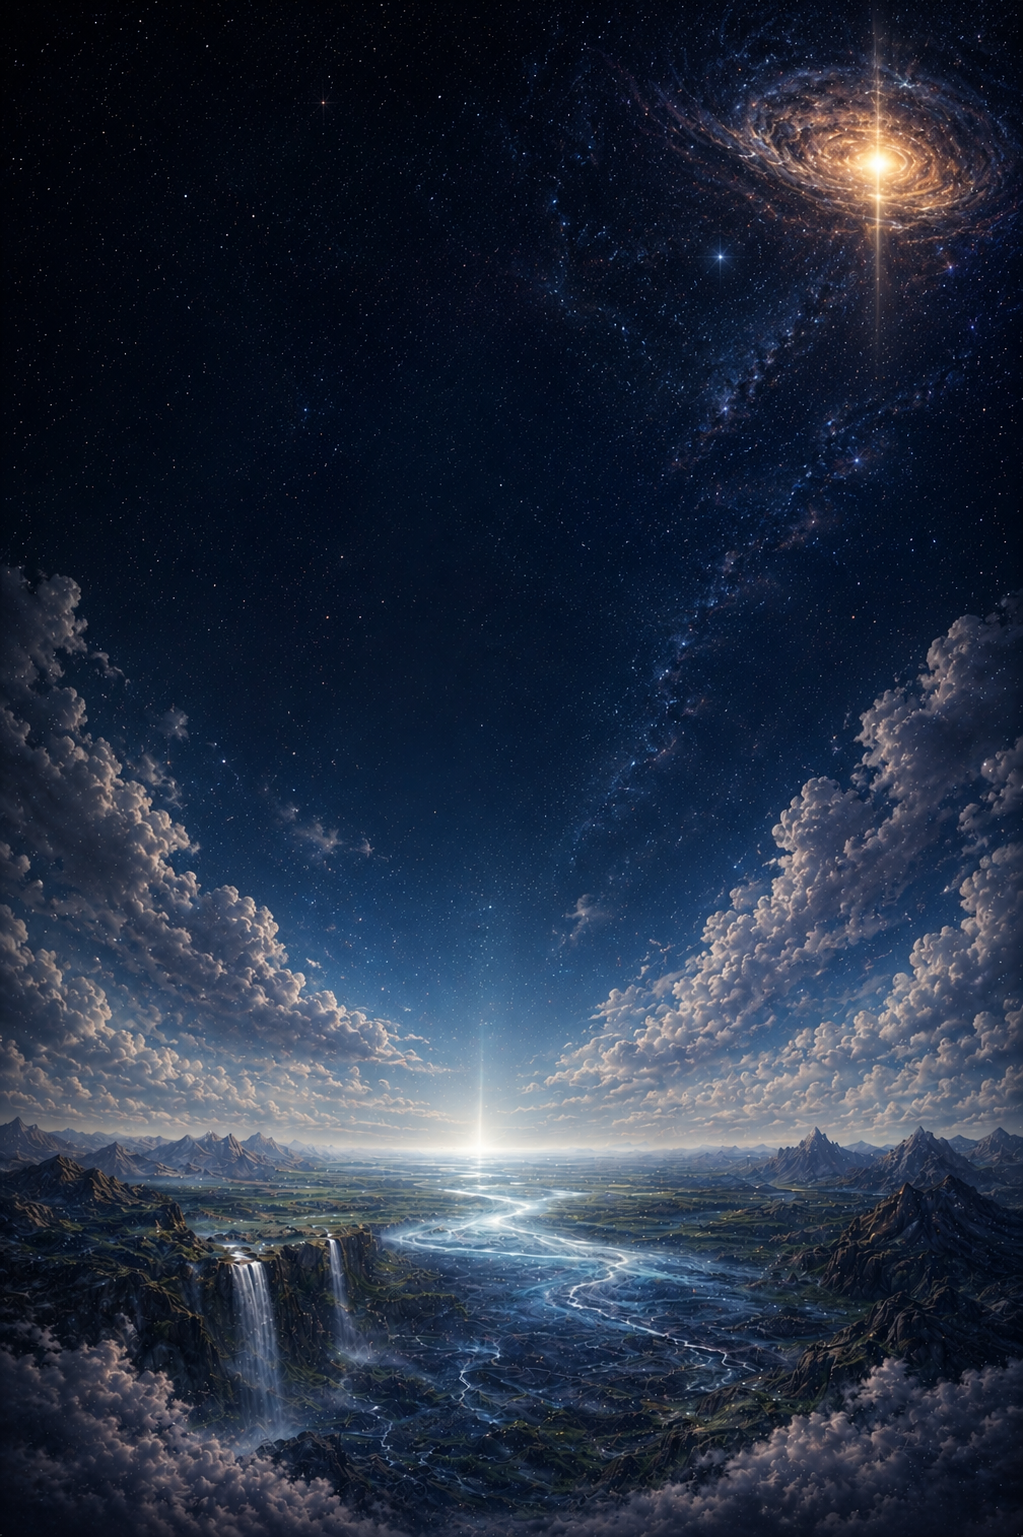
\includegraphics[width=\paperwidth,height=\paperheight]{rueckseite.png}}
}

% --- Safe-Area Offsets ---
\newlength{\bleed}\setlength{\bleed}{0.125in}
\newlength{\safe}\setlength{\safe}{0.35in}
\newlength{\inset}\setlength{\inset}{\dimexpr\bleed+\safe\relax} % = 0.475in

\begin{document}
	\thispagestyle{empty}
	
	% -------------------------------------------------
	% Rückseitentext absolut positioniert
	% -------------------------------------------------
	
\begin{tikzpicture}[remember picture,overlay]
		\node[
		anchor=north west,
		inner sep=0pt,
		text width=4.25in,
		align=justify
		] at ([xshift=1.0in,yshift=-1.50in]current page.north west) {%
			
			% Titel
			{\color{coveraccent}\fontsize{17}{21}\selectfont\bfseries\sffamily
				Die Struktur der Welt\par}
			
			\vspace{0.45em}
			
			% Fließtext
			{\color{covertext}
				\fontsize{11.2}{15.0}\selectfont
				\sffamily
				\spaceskip=0.38em plus 0.16em minus 0.08em
				
				Ist Mathematik nur ein Werkzeug des Menschen -- oder beschreibt sie eine tiefere Ordnung der Wirklichkeit?
				Dieses Buch führt von den Zahlen über Geometrie, Naturgesetze, Wahrscheinlichkeit und moderne Physik
				bis zur Frage, warum die Welt überhaupt mathematisch verstehbar ist.
				
				\medskip
				
				Mathematik erscheint dabei nicht als bloße Rechentechnik, sondern als universelle Struktur:
				sichtbar in Formen, Bewegungen, Symmetrien, Naturgesetzen und den Grenzen unseres Denkens.
				
				\medskip
				
				\textbf{Für interessierte Leserinnen und Leser, die Mathematik nicht nur anwenden, sondern wirklich verstehen wollen.}
				
				\medskip
				
				\emph{Christian Weilharter, Dipl.-Ing.(FH),} verbindet Ingenieursdenken,
				mathematische Neugier und physikalische Perspektive.
				Dieses Buch schlägt die Brücke zwischen verständlicher Darstellung,
				wissenschaftlicher Tiefe und philosophischer Reflexion.
			}
		};
	\end{tikzpicture}
	
\end{document}